\documentclass[10pt]{article}
\usepackage[T1]{fontenc}
\usepackage{lmodern,amsmath,amssymb,graphicx,hyperref}
\usepackage[margin=0.75in]{geometry}
\setlength{\parindent}{0pt}\setlength{\parskip}{6pt}
\begin{document}
\begin{center}
{\Large Orientation-guarded anchor completion}\\[4pt]
14 November 2026 --- original rational/2-adic tensor model\\
Source \texttt{a970572ef271aef7c9a6b852413957fb7cff5b9c}
\end{center}

\textbf{Construction.} The public equality-of-bits guard repairs crossings
omitted by the earlier divisibility guard. The actual completion preserves
all source values, has a computed monic quotient and a bounded degree.
This is a source-bound component; all PCC claims are unsigned
[pcc:unverified].

Let $L=2^a$, $S=\{-L,\ldots,L-1\}$,
$C(T)=\prod_{t\in S}(T-t)$, $\kappa=C'(0)$ and $\delta=y-x$, with
$0\le x,y<L$. For retained bits $u\le a$ and $m_j\in\mathbb N$, define
\begin{align*}
 M_{xy}&=\{j<u:\operatorname{bit}_j(x)=\operatorname{bit}_j(y)\},\\
 B_\delta(T)&=\kappa^{-1}\prod_{t\in S\setminus\{\delta\}}(T-t),\\
 F_{xy}(T)&=\prod_{j\in M_{xy}}
 \left(\frac{2^j-T}{2^j-\delta}\right)^{m_j},\\
 Q_{xy}&=(F_{xy}-1)\mathbin{\mathrm{divMonic}}(T-\delta),\qquad
 H_{xy}=\kappa^{-1}Q_{xy},\\
 W_{\mathrm{new}}[x,y]&=B_\delta F_{xy}.
\end{align*}
All polynomial coefficients here are rational numbers.

\textbf{Exact completion proof.} If $\delta=2^j$, adding $2^j$ flips bit
$j$, including carries. Thus selected denominators are nonzero. Every
selected factor evaluates to one at $\delta$, so the computed monic
remainder is zero and $F_{xy}-1=(T-\delta)Q_{xy}$. Since
$C=(T-\delta)\prod_{t\ne\delta}(T-t)$,
\[
 W_{\mathrm{new}}[x,y]-B_\delta=C H_{xy}.
\]
The nodal polynomial vanishes at every old node, preserving every source
value. Its derivative at zero is a product of nonzero differences, so
$\kappa\ne0$. At zero the matrix remains the identity. No nonscalar-origin
channel is constructed. PCC-20261114-347a54 [pcc:unverified].

\textbf{Degree budget.} Put $M=\sum_{j<u}m_j$, including unused anchors.
Then $\deg F_{xy}\le M$, $\deg W_{\mathrm{new}}\le2L-1+M$ and
$\deg H_{xy}<M$. Zero has degree $-\infty$ and is included. Hence
$M\le2L$ meets the original completion window $\deg H\le2L-1$.
Removed-node membership is explicit and derived from bounded actual indices.
PCC-20261114-278ad6 and proof-map degree entries [pcc:unverified].

\textbf{Prior work.} The repeated-anchor study already derived diagonal
Fibonacci schedule costs and exhibited the missed crossing $(x,y)=(0,1)$ at
level $i=1$. Its guard $2^{j+1}\mid\delta$ omits that pair's anchors.
The new guard includes level1 for that crossing, analytically for every
$u>1$. No novelty is claimed for interpolation, elementary valuations,
Fibonacci schedules or the earlier anchor family.

\newpage
\begin{center}{\Large Actual coefficientwise content}\end{center}

\textbf{Denominators.} For $x\ne y$ let $s=v_2(\delta)$. Divisibility by
$2^s$, failure at $2^{s+1}$ and binary remainders imply that bit $s$ differs
and every lower bit agrees. Thus $s\notin M_{xy}$ and, for every selected
$j$,
\[
 v_2(2^j-\delta)=\min(j,s).
\]
At diagonal entries the denominator valuation is exactly $j$; using $s=u$
represents all selected denominators because $j<u$.
This bridge follows actual bits and actual signed differences, rather than
assuming favorable valuations. PCC-20261114-d1c39d [pcc:unverified].

\textbf{Numerators.} At $T=t+2^{a+1}Z$, take nonzero integer $t$ with
$i=v_2(t)\le a$. For $j\ne i$, both coefficients of $2^j-T$ have valuation
at least $\min(i,j)$. For $j=i$, write $t=2^i k$ with odd $k$;
$2^i-t=2^i(1-k)$ is divisible by $2^{i+1}$ and the linear coefficient has
valuation $a+1$. Thus the numerator has content at least $i+1$.
Zero coefficients have every bound in the formal content predicate.
Finite coefficient sums and products preserve the resulting bounds
[pcc:unverified].

\textbf{Uniform crossing gain.} Define
\[
 b(i,s,j)=
 \begin{cases}i+1,&j=i,\\\min(i,j),&j\ne i\end{cases}
 -\min(s,j),\qquad
 G_i=m_i-\sum_{i<j<u}(j-i)m_j.
\]
At a level-$i$ crossing, bit $i$ agrees, so the mask includes $i$.
Its contribution is at least $m_i$. Lower anchors contribute
nonnegatively; a higher anchor loses at most $(j-i)m_j$, and omitting it
loses nothing. Therefore every coefficient of the actual correction
$F_{xy}(t+2^{a+1}Z)$ has valuation at least $G_i$.
PCC-20261114-7a81c4 [pcc:unverified].

\textbf{All source charts.} At a noncrossing $s\le i$, so every selected
factor has nonnegative content. Above the retained range, $j<u\le i$
again gives nonnegative content. At zero, numerator content is $j$,
at least the denominator valuation. Every nonzero integer source index
has valuation at most $a$, which includes $-L$. Thus feasible $G_i\ge0$
makes the correction integral in every literal source chart.
PCC-20261114-e9d567 [pcc:unverified].

\textbf{Explicit remaining premise.} The completed-matrix theorem currently
assumes the actual base chart has content $k$. It then preserves content $k$,
and every retained crossing has content $k+g$ if $G_i\ge g$. Base content
is an exposed, separate obligation, not an assumed correction gain.
PCC-20261114-8e3afc [pcc:unverified].

\textbf{Cost qualification.} The diagonal schedule is unchanged, so the
older necessary mass $gF_{2u}$ is not evaded. The retained-$u$ statement
cannot be replaced with an all-$a$ obstruction. Masks above $i$ vary within
old tiles; a tile, Walsh or moment refinement needs explicit accounting.
No integral low-rank factorization or recursive cost is established here.

\newpage
\begin{center}{\Large Evidence and next obligation}\end{center}
\begin{center}
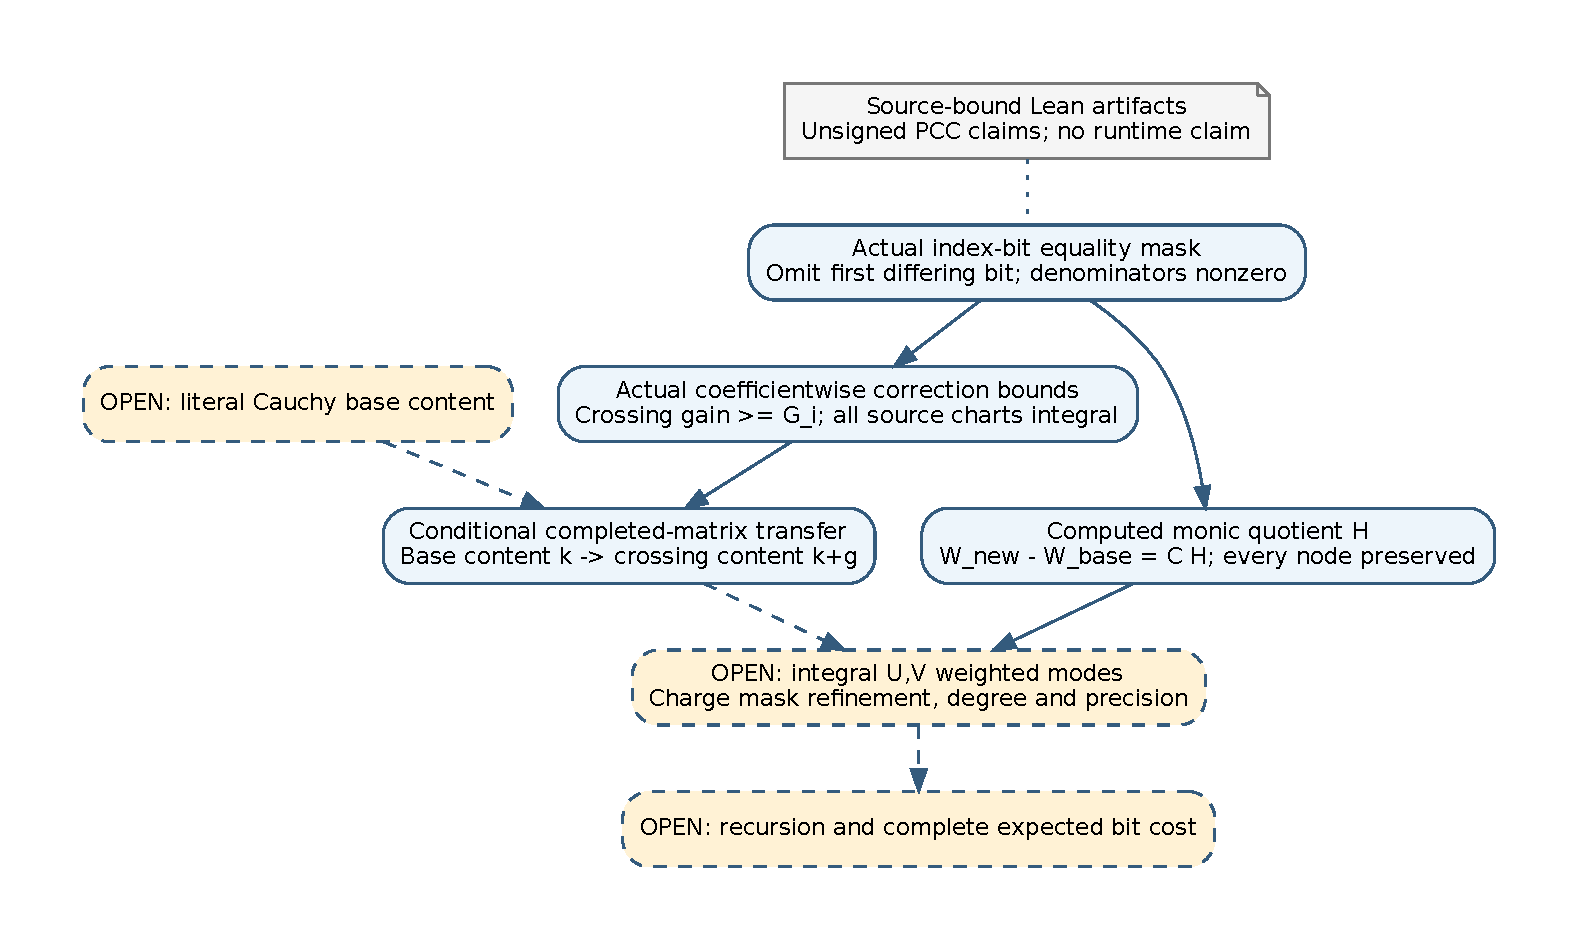
\includegraphics[width=.85\linewidth,height=.52\textheight,keepaspectratio]{construction.pdf}
\end{center}

\textbf{Formal evidence.} Four Lean modules contain 66 authored statements.
The pinned shared proof gate reports 66 theorems and 0 extra trusted axioms.
The import-inclusive fresh replay is still running at this checkpoint.
The evolving evidence and final receipt are linked from the
editable Markdown report. All claims remain unsigned; source binding and
producer checks do not create signed standing [pcc:unverified].

\textbf{Literal certificate.} Certificate \texttt{IDC1h5e866a7c08042f35} checks only
$c p(1+zq)-cp=(pz)(cq)$, a universal ring substep. It does not certify
monic division, bit masks, valuations, rank or the algorithmic objective.
The artifact adapter includes dropped-subtraction and understated-degree
negative controls. Its 25 tests and formatting pass; strict Clippy reports
only unchanged shared SHA256 style errors (4 library, plus 1 test-only).
No timing, solve or scaling experiment is reported.

\textbf{Contract status.} Actual bit/valuation and polynomial construction
are implemented. Absolute Cauchy base content, integral weighted modes,
refinement counts, recursive costs and complete expected bit cost remain
open. The earlier native norm fixture remains unlaunched under its
checkpoint transport blocker. Passing this component does not complete the
broader algorithm objective.

\textbf{Sources and reproducibility.} See the companion Markdown report for
primary files pinned at \texttt{1385553ca}, the prior counterexample,
Fibonacci qualification and search scope. KB unavailable; bounded fallback
search does not establish priority. The proof map lists all exact theorem
hypotheses and unsigned claim identifiers. Failed sources and raw outputs
remain alongside the successful artifacts.

\path{research/prime_orientation_anchor_20261114/PROOF_MAP.md}\\
\path{research/prime_orientation_anchor_20261114/evidence/claim-pins.json}\\
\path{research/prime_orientation_anchor_20261114/evidence/source-freeze.json}

The diagram is explanatory. No performance or solve value is added to the
canonical scoreboard, timeline or norm charts.
\end{document}
